% Illustration and advantages of variable capacity
\begin{slide}[Les PàCCV adaptent leur capacité aux besoins\\
			  pour fonctionner de façon continue]

% Illustration
\only<1>{
\node[anchor=mid west, align=left] at (p5cl cs:1,11) {capacité\\fixe};
\node[anchor=mid west, align=left] at (p5cl cs:1,3) {capacité\\variable};

\begin{scope}[shift={(p5cr cs:1,10)},
			  x=\bigcol/6+\baselineskip/6, y=3\baselineskip]

\draw[semithick] (0,.3333333) -- (3,.33333333) |- (6,.666666);
\draw[col, very thick]
	  (0,0) .. controls (0.1, 1) and (0.2, 1) .. (0.5,1)
   -- (0.5,1) .. controls (0.52, 0) and (0.6, 0) .. (0.7,0)
   -- (1.5,0) .. controls (1.6, 1) and (1.7, 1) .. (2,1)
   -- (2,1) .. controls (2.02, 0) and (2.1, 0) .. (2.2,0)
   -- (3,0) .. controls (3.1, 1) and (3.2, 1) .. (3.5,1)
   -- (4,1) .. controls (4.02, 0) and (4.1, 0) .. (4.2,0)
   -- (4.5,0) .. controls (4.6, 1) and (4.7, 1) .. (5,1)
   -- (5.5,1) .. controls (5.52, 0) and (5.6, 0) .. (5.7,0) -- (6,0);
	
\end{scope}


\node[becomes, rotate=180] at (p5cr cs:2,7.5) {};


\begin{scope}[shift={(p5cr cs:1,2)},
			  x=\bigcol/6+\baselineskip/6, y=\baselineskip]

\draw[semithick] (0,1) -- (3,1) |- (6,2);
\def\phase{46.87329}  % found numerically with scipy
\draw[col, very thick] plot[domain=0:3, samples=100, smooth]
			(\x, {1 - exp(-2*\x) * cos(700*\x + \phase) / cos(\phase)});
	
\end{scope}


\begin{scope}[shift={($(p5cr cs:1,3)+(\colv+\baselineskip,0)$)},
			  x=\bigcol/6+\baselineskip/6, y=\baselineskip]

% use rect line cap for joining but clip the part sticking out
\clip (p5cr cs:1,3) rectangle ++(2\colvsep,3\baselineskip);
\def\phase{46.87329}
\draw[col, very thick, line cap=rect] plot[domain=0:3, samples=100, smooth]
			(\x, {1 - exp(-2*\x) * cos(700*\x + \phase) / cos(\phase)});
\end{scope}
}


% Advantages
\only<2->{
\node[anchor=base west, align=left] (list) at (t5cr cs:1,5){
	\begin{minipage}[b]{2\colvsep}
	\hskip-.8pt Et ainsi elles augmentent\\
	\begin{listed}
        \item la performance
        \item la plage de températures
    \end{listed}
    \end{minipage}};
}

\end{slide}



% Étude de cas
\begin{slide}[Un modèle dynamique adéquat est nécessaire\\
			  pour simuler correctement les PàCCV]

\node[anchor=base west] (text) at (t5cl cs:0,4) {
	\begin{minipage}[b]{\dimexpr2\colvsep+4\quanta}\raggedright
		\emph{Exemple}\\[2\baselineskip]
		Profil de consommation\\d'une unité de résidence typique,\\~\\
		avec un pas de temp $ \Delta t = \SI{1}{\minute} $
	\end{minipage}};

\node[anchor=south east] at (p5cr cs:4,3)
	{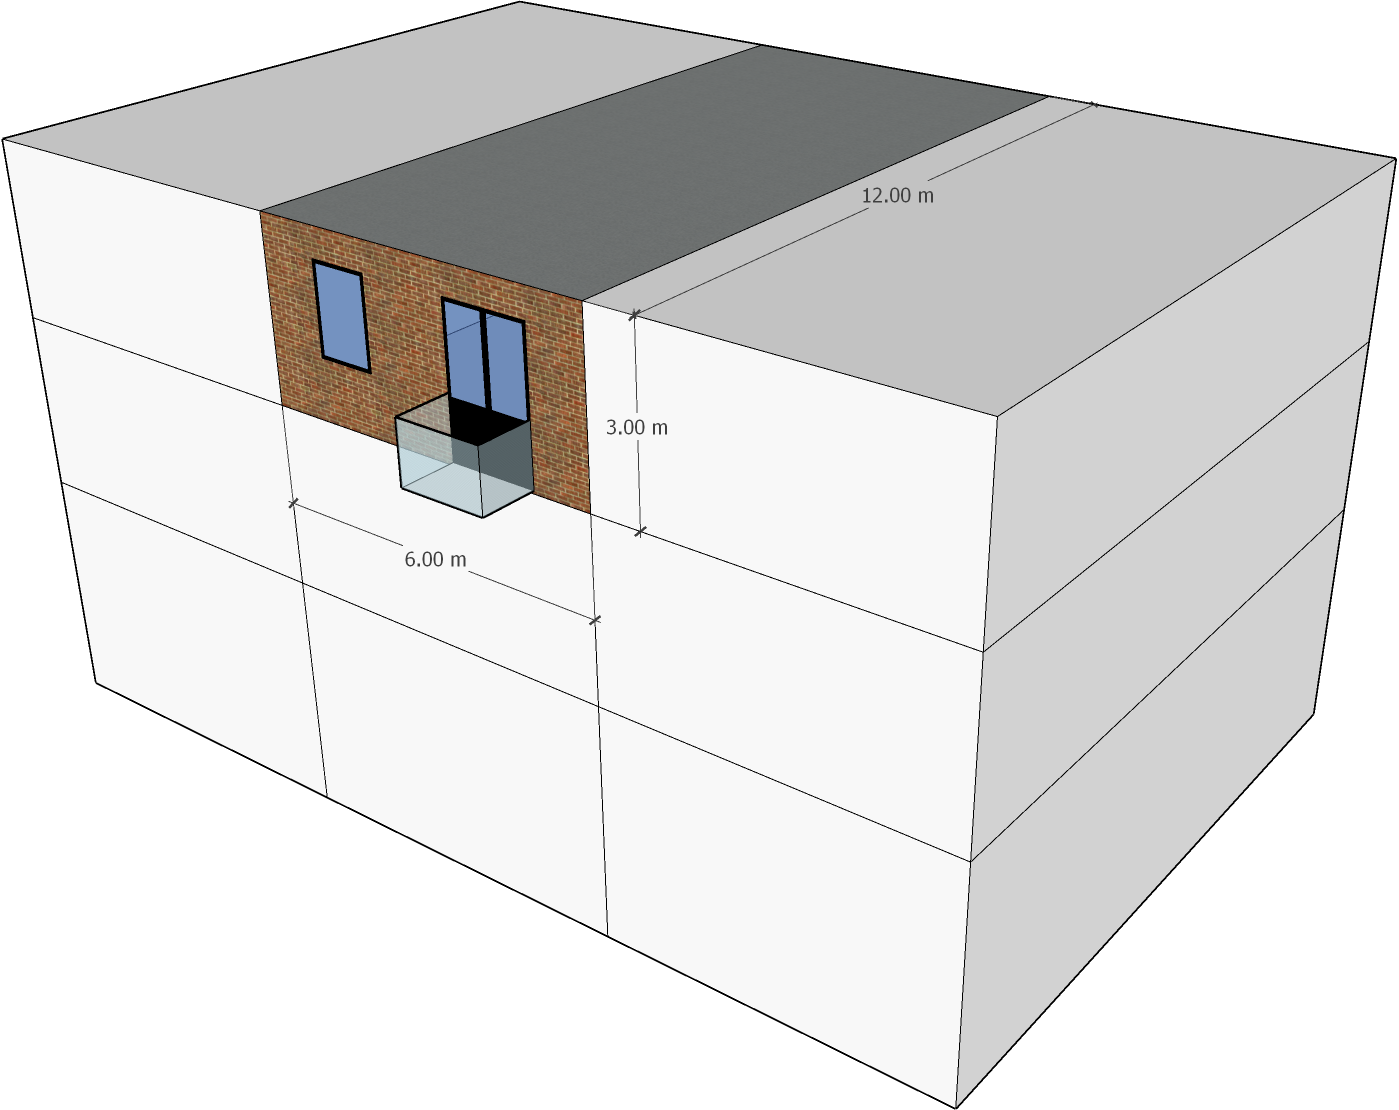
\includegraphics[height=9\baselineskip]{pictures/plex-unit}};

\end{slide}



% Données incomplètes
\begin{slide}[Les manufacturiers ne donnent pas suffisamment\\
			  d'informations sur les performances%
			  \only<5->{, ni sur le contrôle}]

\only<1>{
\begin{axis}[plot options, clip=false,
			 at={(p5cl cs:2,2)},
			 width=\bigcol+2\baselineskip, height=12\baselineskip,
			 xtick={-26.1, 15},
			 xticklabels={\num{-26.1}\phantom{$-$},
			 			  \phantom{\,\si{\celsius}}\SI{15}{\celsius}},
			 ytick={1.42, 4.75},]
\foreach \i in {1, ..., 4}{
	\addplot[mark=*, mark size=1pt, semithick] table[x=Toa, y=COP_at_T\i]
		{data/manu-data-heating.tsv};}
\foreach \i/\COP in {1/4.75, 2/4.524, 3/4.339, 4/3.961}{%
	\edef\temp{\noexpand\node (T\i) at (axis cs:15,\COP) {};}
	\temp}
\end{axis}
\node[anchor=mid west, font=\footnotesize] at (p5cl cs:1,14) {COP};
\node[anchor=base east, font=\footnotesize] (Toa)
	at (t5cr cs:4,0) {\To};
\foreach \i/\Ti in {1/15.6, 2/18.3, 3/21.1, 4/23.8}{
	\node[font=\footnotesize, gray, anchor=east] (Tr\i)
		at (T\i -| Toa.east) {\SI{\Ti}{\celsius}};
	\draw[gray] (T\i)++(4.5pt,0) -- ($(Tr\i.west)-(4pt,0)$);}
\node[anchor=west, yshift=-2\baselineskip, font=\footnotesize]
	at (Tr4.west) {\Tr};
}

\def\displayat{2}
\foreach \row/\rowlabel in {0/3, 1/2, 2/1}{
	\foreach \col/\collabel in {2/1, 3/2, 4/3}{
		\colorlet{background}{gray!10}
		\ifnum \row=2
			\ifnum \col=2
				\temporal<3>{
					\colorlet{background}{gray!10}}{
					\colorlet{background}{gray!10}}{
					\colorlet{background}{col!20}}
			\fi
		\fi
		\ifnum \col=2
			\renewcommand\displayat{2}
		\else
			\renewcommand\displayat{3}
		\fi
		\begin{axis}[visible on=<\displayat-4>,
					 enlargelimits=false, scale only axis,
					 hide axis,
					 at={($(p5cl cs:\col,0)+(0,56*\row*\quantum/3)$)},
					 width=\colv, height=11\baselineskip/3,
					 axis background/.style={fill=background}]
		
		\foreach \i in {1, ..., 4}{
			\addplot[mark=*, mark size=.5pt] table[x=Toa, y=COP_at_T\i]
				{data/manu-data-heating.tsv};}
			
		\end{axis}
		\ifnum \row=0
			\node[xshift=.5\colv, anchor=base, visible on=<3-4>]
				at (p5cl cs:\col,14){\ma[\collabel]};
		\fi
	}
	\pgfmathparse{2+\row}\let\labelypos\pgfmathresult
	\node[anchor=east, visible on=<2-4>] (row\row)
		at ($(p5cr cs:1,0)+(0,{(22+56*\row)*\quantum/3})$)
		{\fc[\rowlabel]};
}

\node[anchor=base] (pct) at ($(t5cl cs:0,6)!0.5!(row1.base west)$)
	{$ {\uncover<4>{{\color{col}1}\above 0.4pt} \uncover<3-4>{3 \times 3}}
	   \uncover<4>{\approx \SI{11}{\percent}} $};

\uncover<3-4>{
	\node[align=left, font=\footnotesize] (required)
		at (pct.202 |- row0) {paires $ (f, \dot m) $\\nécessaires};
	\draw (pct.202)++(0,-4pt) -- ($(required.north)+(0,4pt)$);}
\uncover<4>{
	\node[align=left, font=\footnotesize] (provided)
		at (pct.158 |- row2) {paire $ (f, \dot m) $\\fournie};
	\draw[col] (pct.158)++(0,4pt) -- ($(provided.south)-(0,4pt)$);}


\node[anchor=base west, align=left, visible on=<5>] at (t5cr cs:1,2){
	\begin{minipage}[b]{3\colvsep}\raggedright
	\hskip-.8pt Beaucoup de ``cas spéciaux'' sont détaillés,\\~\\
	\begin{listed}
		\item les limites d'opération\\
			  {\footnotesize\color{gray} fréquences minimale et maximale,
			  							 \ldots}
		\item le contrôle des ventilateurs\\
			  {\footnotesize\color{gray} vitesse en fonction
			  							 de la température}
		\item le contrôle du mode d'opération\\
			  {\footnotesize\color{gray} chauffage ou climatisation,
			  							 selon la consigne}
	\end{listed}
	\vskip\baselineskip \hskip-.8pt mais pas le contrôle normal
									de la fréquence 
	\end{minipage}};

\end{slide}



\begin{slide}[Les stratégies de contrôle et les performances\\ 
			  sont évaluées expérimentalement]

\node[anchor=north west] at (p5cl cs:.25,15)	{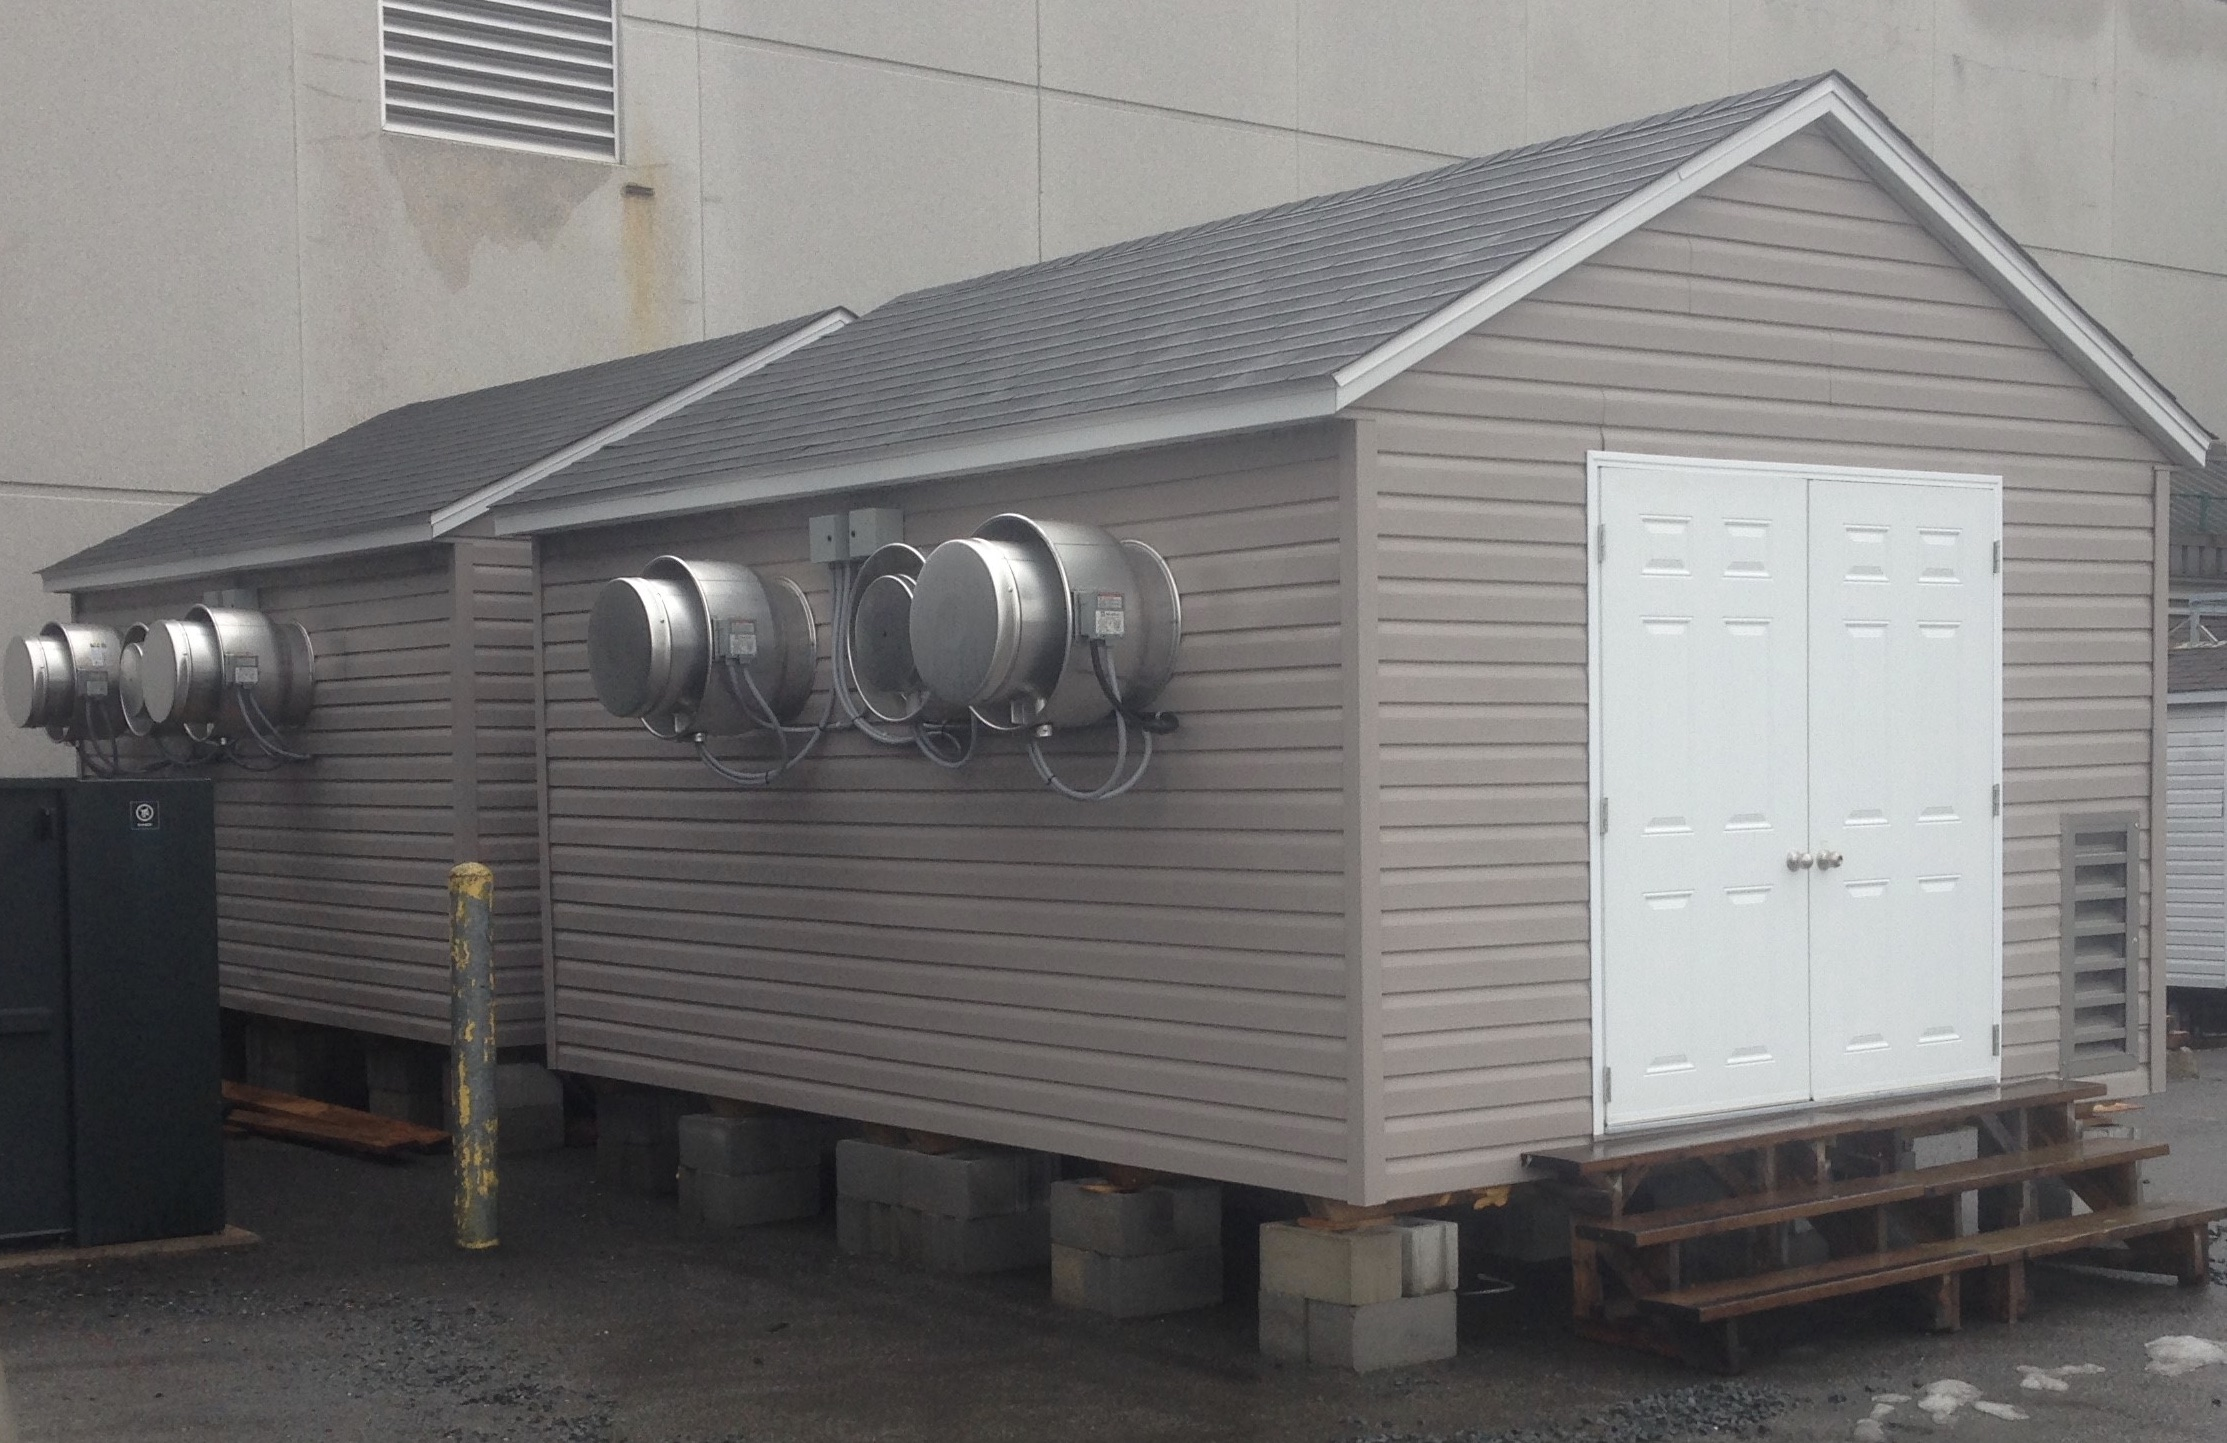
\includegraphics[width=2\colvsep]{pictures/sheds}};
\node[anchor=south west] at (p5cl cs:.25,0)
	{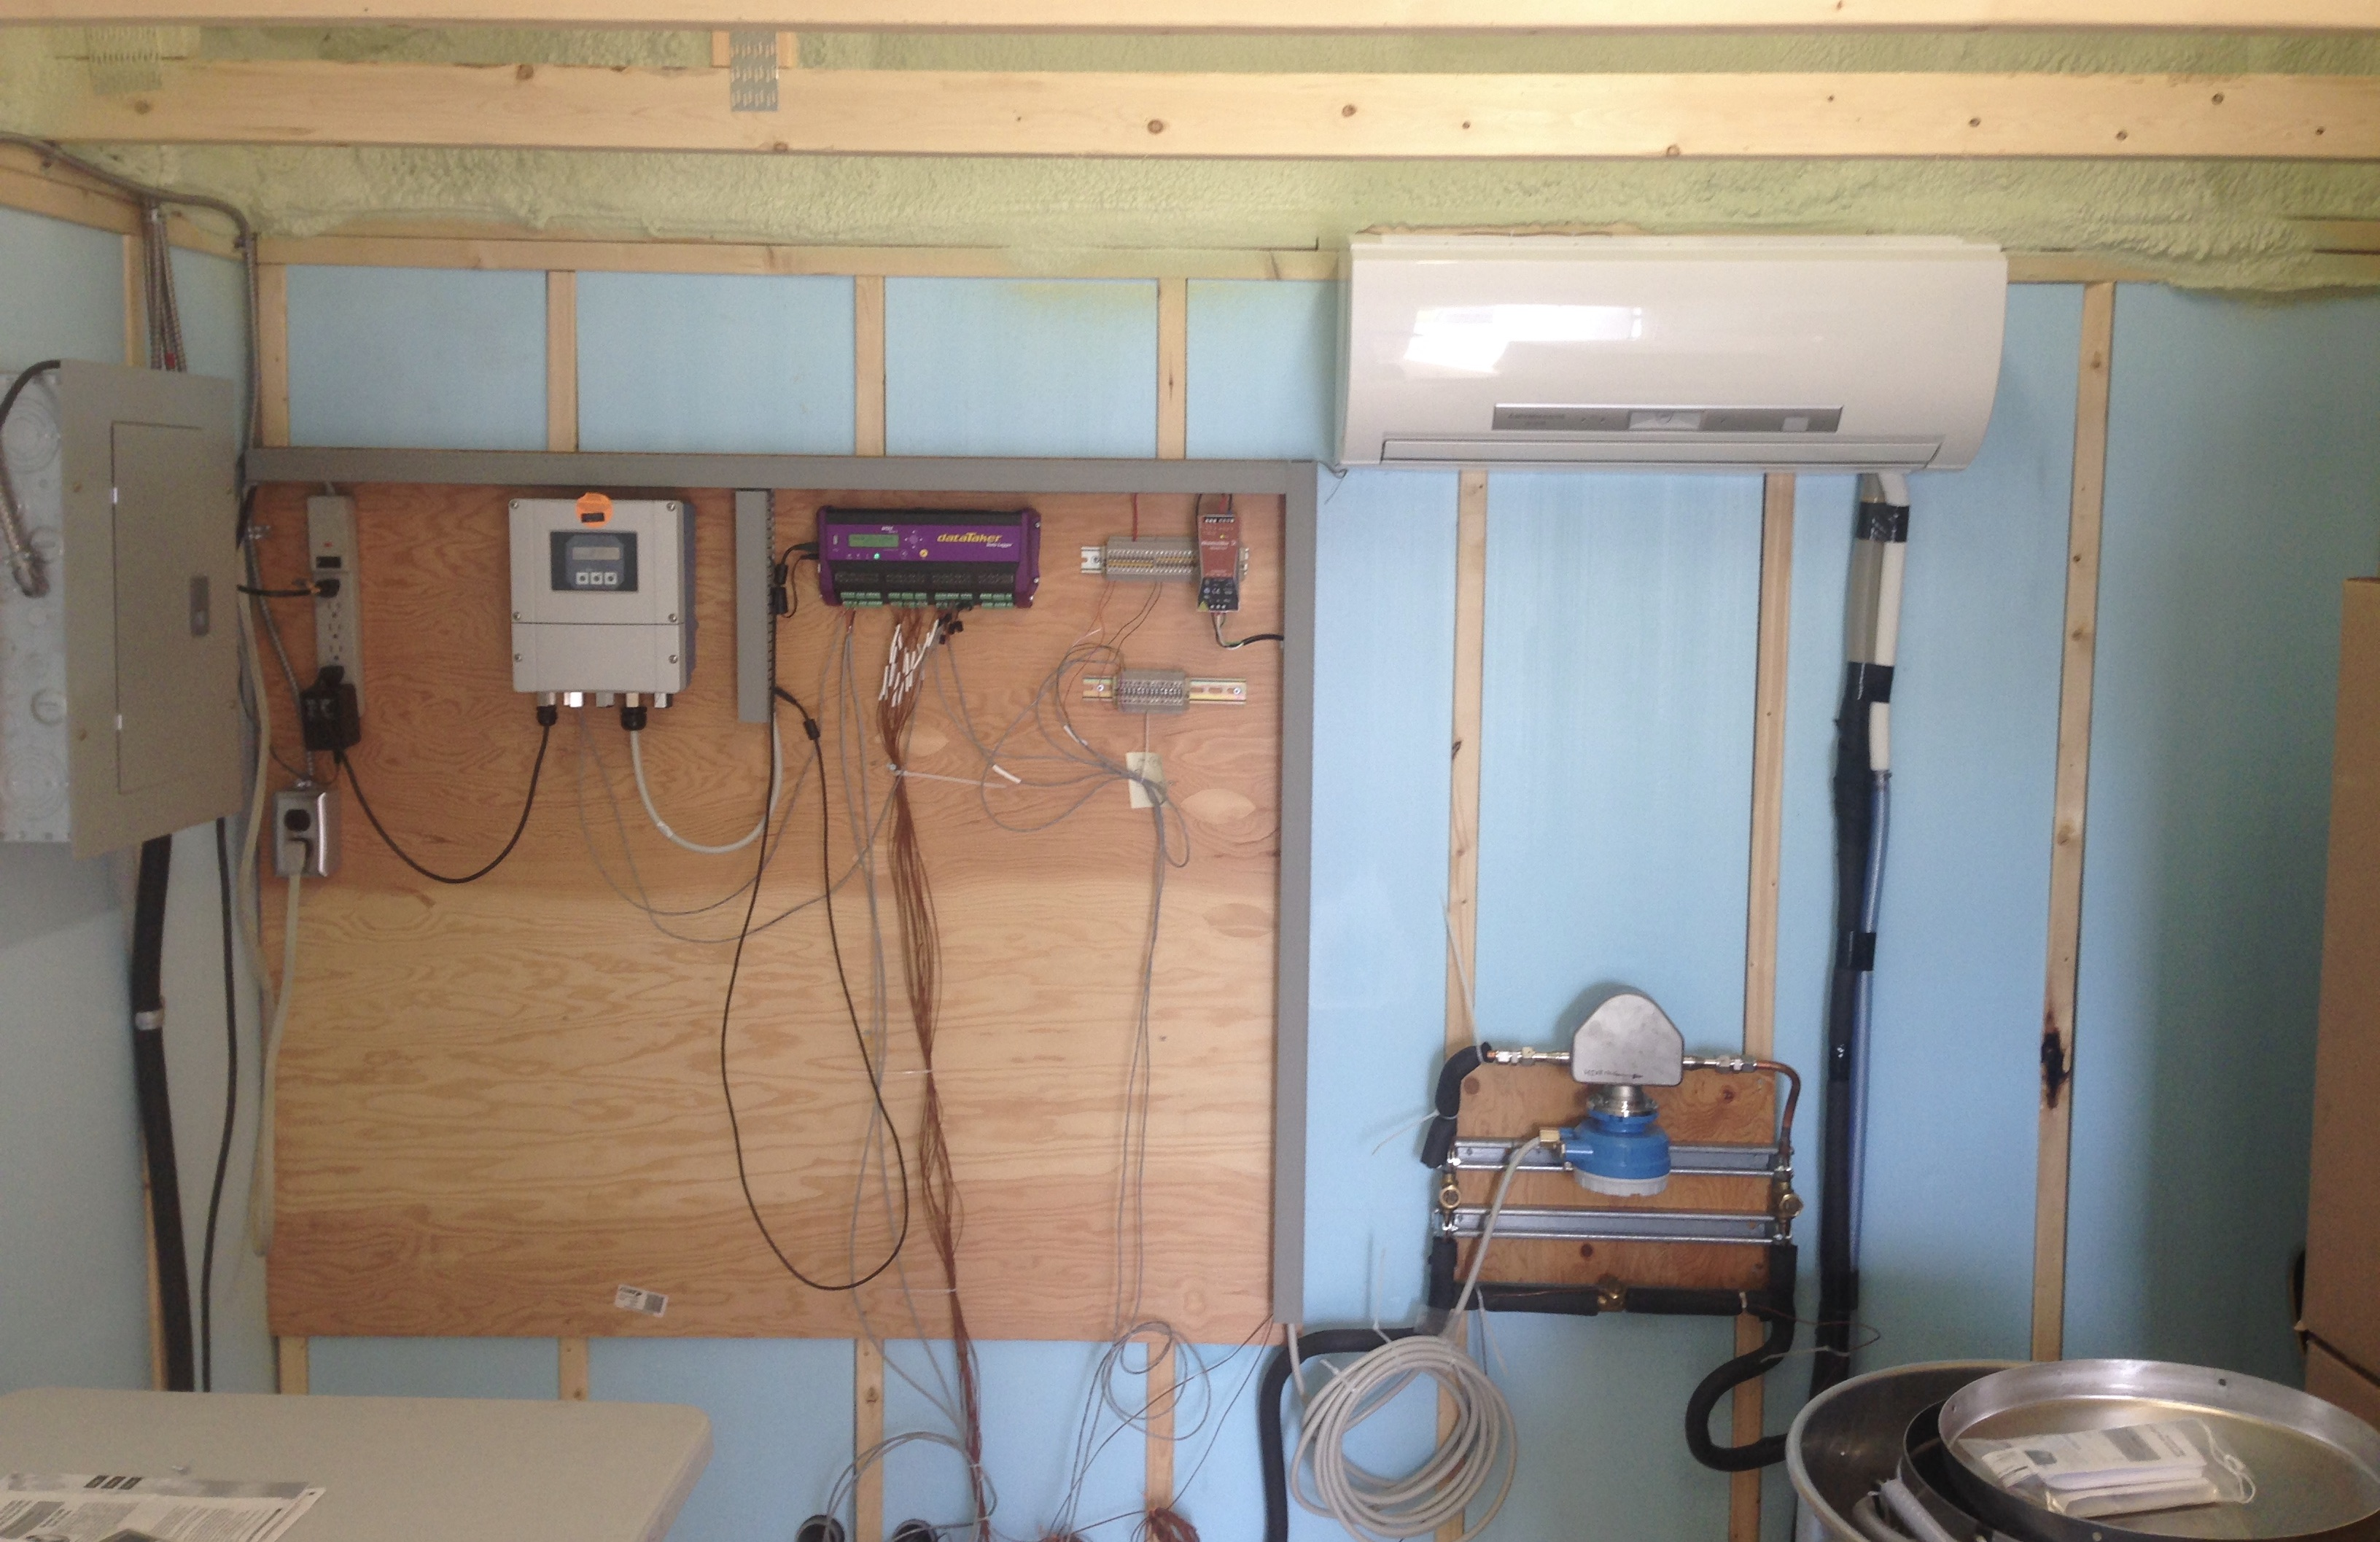
\includegraphics[width=2\colvsep]{pictures/indoor-unit}};
\node[anchor=south east] at (p5cr cs:3.75,0)
	{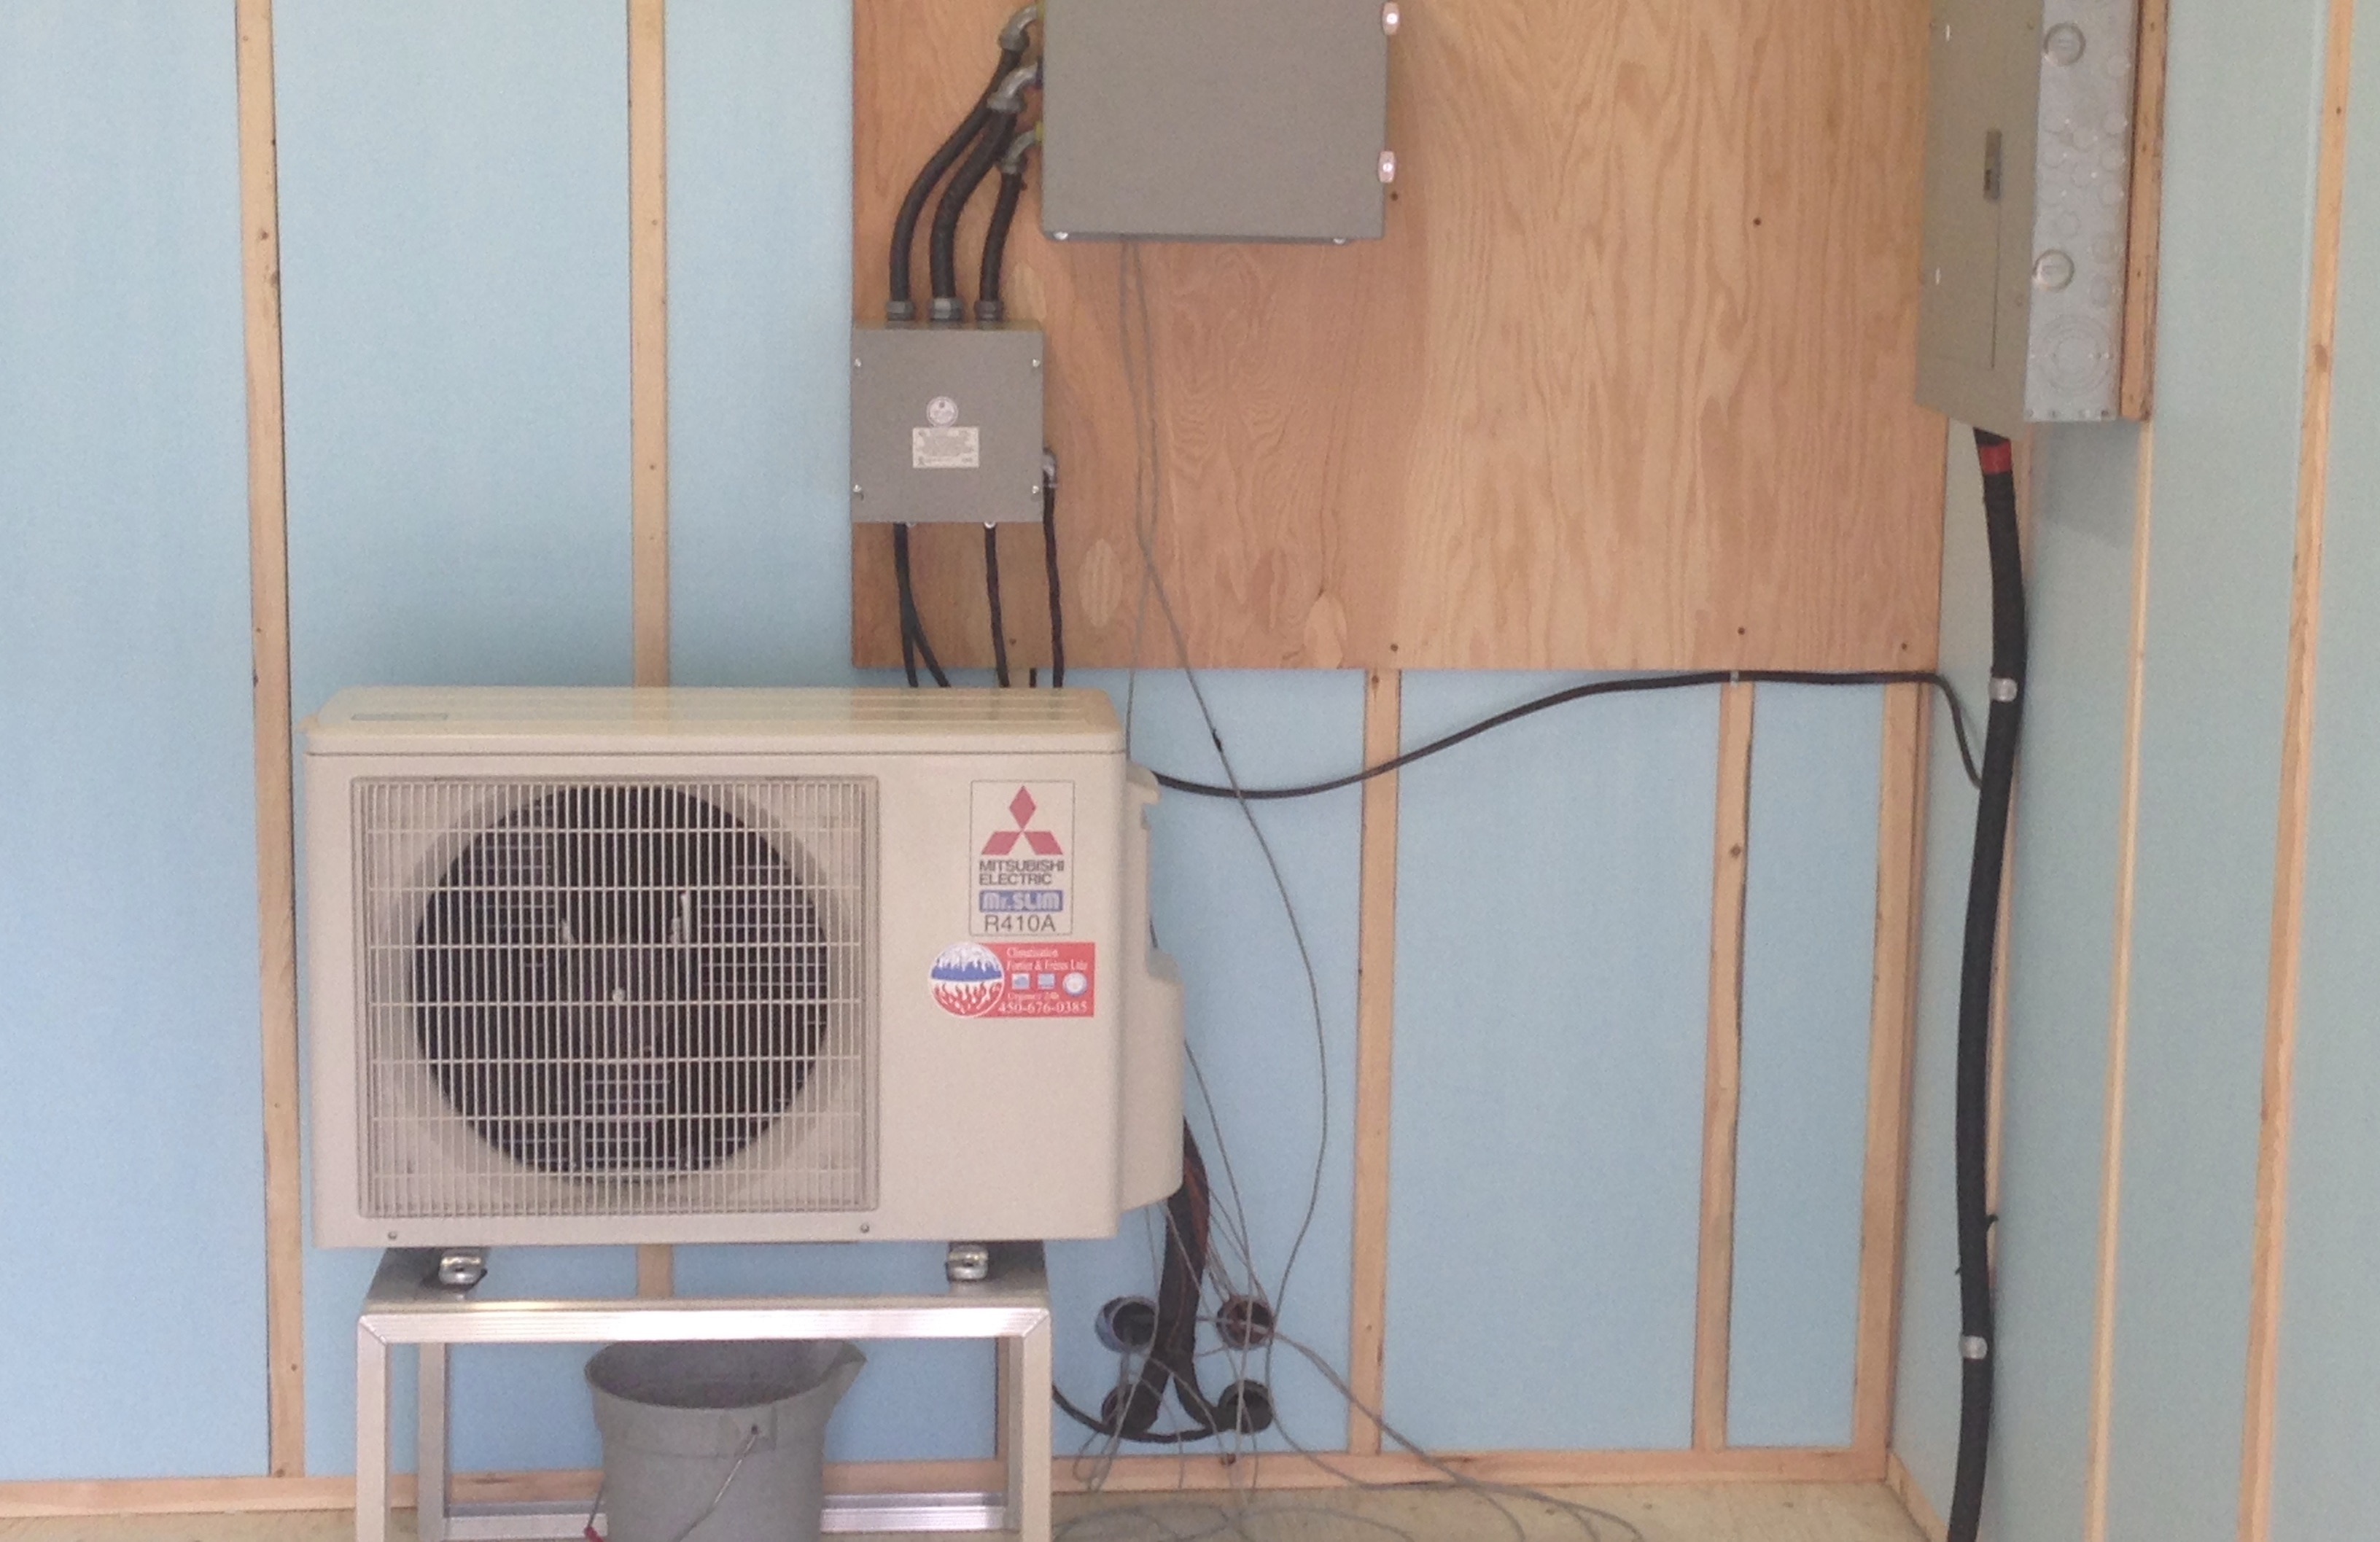
\includegraphics[width=2\colvsep]{pictures/outdoor-unit}};

\node[anchor=base east] at (t5cr cs:3.75,8){
	\begin{minipage}[b]{2\colvsep}
		Pour obtenir les performances dans les conditions désirées,
		\begin{listed}
		\setlength\itemsep{0pt}
			\item la charge
			\item la température extérieure
			\item le débit d'air
		\end{listed}
		sont imposés en contrôlant la quantité d'air entrant
	\end{minipage}};

\end{slide}



\begin{slide}[Le modèle parvient à prévoir les performances\\
			  \only<2>{et à reproduire les principaux comportements}]

\only<1>{
\begin{groupplot}[group style={group size=1 by 2,},
				  width=\bigcol+\colvsep,
				  xmin=0, xmax=3,
				  clip=false,
				  plot options,]
\nextgroupplot[
	height=3\baselineskip,
	axis x line=none,
	ymin=3.5, ymax=3.8,
	ytick={3.5, 3.8},
	yticklabels={3.5,\SI{3.8}{\kilo\watt}},
	at={(p5cr cs:1,10)},
	anchor=south west,
	]
\addplot[thick, gray] table[x=TIME, y=Qc-exp] {data/cooling-io.tsv};
\addplot[thick,  col] table[x=TIME, y=Qc-sim] {data/cooling-io.tsv};
\draw[latex-] (axis cs:1.7, 3.76) |- ++(3\quanta, 4\quanta)
	node[right, inner sep=3pt] {\footnotesize \SI{6.5}{\percent} error};
\draw[latex-] (axis cs:1.7, 3.5148) |- ++(0mm, -4\quanta);

\nextgroupplot[
	height=3\baselineskip,
	xtick={0, 3},
	xticklabels={0, \phantom{h\,}\SI{3}{\hour}},
	ymin=0.84, ymax=0.94,
	ytick={0.84, 0.94},
	yticklabels={840,\SI{940}{\watt}},
	at={(p5cr cs:1,3)},
	anchor=south west,
	]
\addplot[thick, gray] table[x=TIME, y=Pel-exp] {data/cooling-io.tsv};
\addplot[thick, col] table[x=TIME, y=Pel-sim] {data/cooling-io.tsv};
\draw[latex-] (axis cs:0.5833, 0.91648) |- ++(3\quanta, 4\quanta)
	node[right, inner sep=3pt] {\footnotesize \SI{8}{\percent} error};
\draw[latex-] (axis cs:0.5833, 0.84669) |- ++(0mm, -4\quanta);

\end{groupplot}

\node[anchor=mid west] at (p5cr cs:0,13) {\footnotesize\Qc};
\node[anchor=mid west] at (p5cr cs:0,6) {\footnotesize\Pel};
\node[gray, anchor=base west] at (t5cr cs:1.4,13.5)
	{\scriptsize measurements};
\node[col, anchor=base west] at (t5cr cs:1.4,9) {\scriptsize simulation};
}


\only<2>{
\begin{groupplot}[group style={group size=1 by 3,},
				  width=\bigcol+\colvsep,
				  xmin=0, xmax=4,
				  clip=false,
				  plot options,]
\nextgroupplot[
	height=3\baselineskip,
	axis x line=none,
	ymin=0, ymax=57,
	ytick={0, 57},
	yticklabels={0, \SI{57}{\hertz}},
	at={(p5cr cs:1,11)},
	anchor=south west,
	]
\addplot[thick, gray] table[x=TIME, y=f-exp] {data/cooling-sim.tsv};
\addplot[thick, col] table[x=TIME, y=f-sim] {data/cooling-sim.tsv};


\nextgroupplot[
	height=2\baselineskip,
	axis x line=none,
	ymin=14, ymax=24,
	ytick={14, 24},
	yticklabels={14, \SI{24}{\celsius}},
	at={(p5cr cs:1,7)},
	anchor=south west,
	]
\addplot[thick, gray] table[x=TIME, y=Ts-exp] {data/cooling-sim.tsv};
\addplot[thick, col] table[x=TIME, y=Ts-sim] {data/cooling-sim.tsv};
\draw[latex-] (axis cs:2.6, 17.373) |- ++(3\quanta, 4\quanta)
	node[right, inner sep=3pt] {\footnotesize\SI{3.7}{\celsius}};
\draw[latex-] (axis cs:2.6, 13.689) -- ++(0mm,-4\quanta);


\nextgroupplot[
	height=3\baselineskip,
	xtick={0, 4},
	xticklabels={0, \phantom{h\,}\SI{4}{\hour}},
	ymin=23, ymax=44,
	ytick={23, 44},
	yticklabels={23, \SI{44}{\celsius}},
	at={(p5cr cs:1,2)},
	anchor=south west,
	]
\addplot[thick] table[x=TIME, y=Toa] {data/cooling-sim.tsv}
	node[pos=0.7, fill=white, font=\footnotesize, inner sep=3pt] {\To};
\addplot[thick, gray] table[x=TIME, y=Tr-exp] {data/cooling-sim.tsv};
\addplot[thick, col] table[x=TIME, y=Tr-sim] {data/cooling-sim.tsv};

\end{groupplot}

\node[anchor=mid west] at (p5cr cs:0,14) {\footnotesize\fc};
\node[anchor=mid west] at (p5cr cs:0,9) {\footnotesize\Ts};
\node[anchor=mid west] at (p5cr cs:0,5) {\footnotesize\Tr};
}


\end{slide}
